%% Los cap'itulos inician con \chapter{T'itulo}, estos aparecen numerados y
%% se incluyen en el 'indice general.
%%
%% Recuerda que aqu'i ya puedes escribir acentos como: 'a, 'e, 'i, etc.
%% La letra n con tilde es: 'n.

\chapter{Propuesta}
Se propone un abordaje basado en la t\'ecnicas de procesamiento de imagenes que servir\'an para implementar el sistema de visi\'on global, el cual tendr\'a como salida la posici\'on y orientaci\'on actual en cada frame del robot. Luego de este proceso se utilizar\'a una red neuronal  que aprender\'a de los estados y las posiciones y predecir\'a los siguientes estados para hacerle el seguimiento.\\
Para esto utilizamos marcas encima de los robots, las cuales nos dan mas facilidades para realizar la identificaci\'on de cada robot como se muestra en la Fig \ref{fig_mar}.
	\begin{figure}
	\centering
	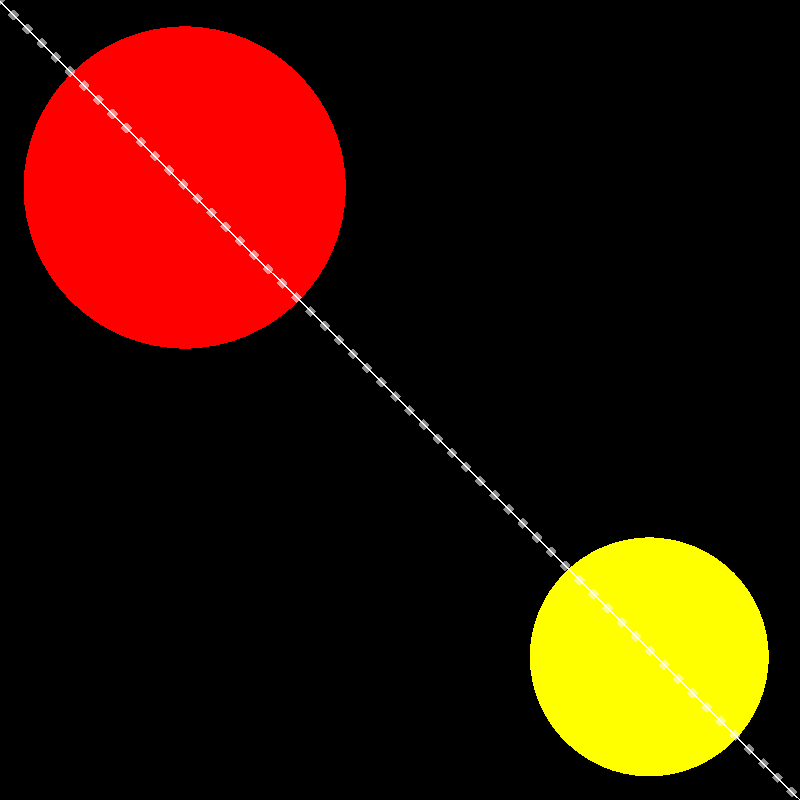
\includegraphics[width=2.5in]{imagen1.pdf}
	
	\caption{Marcas en cada robot}
	\label{fig_mar}
\end{figure}
\section{Sistema de Visi\'on}
En el sistema de vision proponemos utilizar los m\'etodos de el filtro de Gauss y la transformada de Hough. Para realizar esto utilizamos la libreria de OpenCv, la cual nos da soporte para primero aplicar un filtro de gauss para eliminar el ruido en nuestra imagen, luego convertimos nuestra imagen a la escala de grises, y finalmente aplicamos la transformada de Gauss para obtener los c\'irculos en la imagen, cuyos centros tambien son hallados.\\
Una vez hallados los centros y radios de cada circulo procedemos a realizar el calculo de la ubicacion de nuestro robot, el cual utilizara unos circulos marcados como se muestra en la Fig  \ref{fig_cir}. Entonces como tenemos dos circulos de ubicacion conocida procedemos a aplicar el metodo  que nos dice que la posicion basado en esos dos circulos estara en el punto medio de la recta que une los dos centros  $c_i$ y $c_j$ de los dos circulos \cite{kelson_glo}. Entonces aplicamos la siguiente igualdad:
\begin{equation}
cos(\theta)=\frac{y_1-y_2}{a} \qquad; cos(\theta)=\frac{y-y_2}{\frac{a}{2}}
\end{equation}
de la misma manera se puede hallar la coordenada $y$:
\begin{equation}
sen(\theta)=\frac{x_1-x_2}{a} \qquad; sen(\theta)=\frac{x_2-x}{\frac{a}{2}}
\end{equation}
Entonces al igual las ecuaciones anteriores, se puede hallar la posicion actual del robot la cual es:
\begin{equation}
x=x_2-\frac{1}{2}\cdot ({y_1-y_2} )\qquad ; y=y_2+ \frac{1}{2}\cdot( {x_1-x_2})
\end{equation}
Una vez hallada la posicion actual del robot procedemos a hallar la orientacion con respecto al eje inicial del la imagen, de la misma forma utilizamos un metodo ya utilizado anterioremente,  el cual consiste en comparar los puntos centrales y con su tangente hallar la orientacion (angulo)\cite{kelson_glo}. El angulo $\theta$ de orientacion seria dado por:
\begin{equation}
\theta=arctan(\frac{y_1-y_2}{x_1-x_2} )
\end{equation}

\begin{figure}
\centering
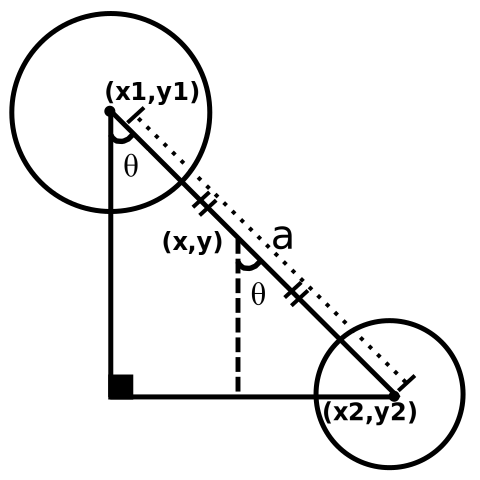
\includegraphics[width=2.5in]{imagen2.pdf}
\caption{C\'alculo de la posici\'on}
\label{fig_cir}
\end{figure}
Asi ya tenemos la posici\'on actual en cada frame y la orientaci\'on que sigue cada robot, y estamos preparados para darle estos par\'ametros a la red neuronal  y se pueda predecir su siguiente posici\'on.
